\subsection{Variando el valor de c}

Antes de realizar cualquier experimentación nos pareció que un valor de $c=0.8$ era muy razonable, ya que respeta las condiciones
originales del problema. El navegante de la web normalmente sigue los links de las páginas, y en alguna que otra ocasión decide
introducir una nueva url.

Al disminuír el valor de $c$, y por lo tanto aumentar el de $(1-c)$, lo que estamos haciendo en realidad es homogeneizar los valores
del vector estacionario final, ya que aumentan las probabilidades de realizar saltos aleatorios. Cuando esto sucede, disminuye
la probabilidad de que un navegante de la web permanezca en una única pág.

Por el contrario, cuando $c=1$ se respeta por completo la instancia inicial, y la diferencia entre el máximo y el mínimo módulo
de los elementos del vector estacionario va a ser menor.

\begin{figure}[!h]
        \begin{center}
                  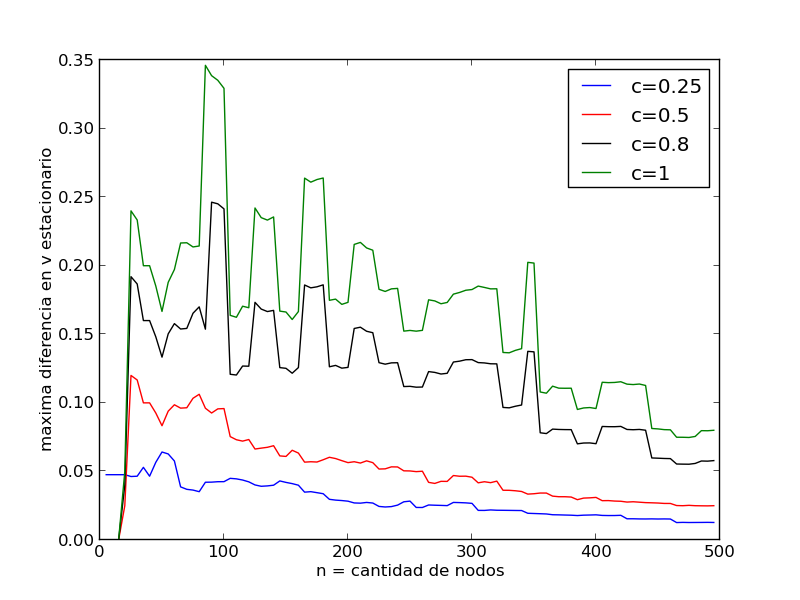
\includegraphics[scale = 0.6]{graficos/variando_c.png}
                  \caption{Variacion entre max y min módulo para distintos valores de c}
                  \label{fig:contra1}
        \end{center}
\end{figure}
\FloatBarrier
